\documentclass[11pt]{article}

    \usepackage[breakable]{tcolorbox}
    \usepackage{parskip} % Stop auto-indenting (to mimic markdown behaviour)
    \usepackage{subcaption}
    \usepackage{iftex}
    \ifPDFTeX
    	\usepackage[T1]{fontenc}
    	\usepackage{mathpazo}
    \else
    	\usepackage{fontspec}
    \fi

    % Basic figure setup, for now with no caption control since it's done
    % automatically by Pandoc (which extracts ![](path) syntax from Markdown).
    \usepackage{graphicx}
    % Maintain compatibility with old templates. Remove in nbconvert 6.0
    %\let\Oldincludegraphics\includegraphics
    % Ensure that by default, figures have no caption (until we provide a
    % proper Figure object with a Caption API and a way to capture that
    % in the conversion process - todo).
    %\usepackage{caption}
    %\DeclareCaptionFormat{nocaption}{}
    %\captionsetup{format=nocaption,aboveskip=0pt,belowskip=0pt}

    \usepackage[Export]{adjustbox} % Used to constrain images to a maximum size
    \adjustboxset{max size={0.9\linewidth}{0.9\paperheight}}
    \usepackage{float}
    \floatplacement{figure}{H} % forces figures to be placed at the correct location
    \usepackage{xcolor} % Allow colors to be defined
    \usepackage{enumerate} % Needed for markdown enumerations to work
    \usepackage{geometry} % Used to adjust the document margins
    \usepackage{amsmath} % Equations
    \usepackage{amssymb} % Equations
    \usepackage{textcomp} % defines textquotesingle
    % Hack from http://tex.stackexchange.com/a/47451/13684:
    \AtBeginDocument{%
        \def\PYZsq{\textquotesingle}% Upright quotes in Pygmentized code
    }
    \usepackage{upquote} % Upright quotes for verbatim code
    \usepackage{eurosym} % defines \euro
    \usepackage[mathletters]{ucs} % Extended unicode (utf-8) support
    \usepackage{fancyvrb} % verbatim replacement that allows latex
    \usepackage{grffile} % extends the file name processing of package graphics 
                         % to support a larger range
    \makeatletter % fix for grffile with XeLaTeX
    \def\Gread@@xetex#1{%
      \IfFileExists{"\Gin@base".bb}%
      {\Gread@eps{\Gin@base.bb}}%
      {\Gread@@xetex@aux#1}%
    }
    \makeatother

    % The hyperref package gives us a pdf with properly built
    % internal navigation ('pdf bookmarks' for the table of contents,
    % internal cross-reference links, web links for URLs, etc.)
    \usepackage{hyperref}
    % The default LaTeX title has an obnoxious amount of whitespace. By default,
    % titling removes some of it. It also provides customization options.
    \usepackage{titling}
    \usepackage{longtable} % longtable support required by pandoc >1.10
    \usepackage{booktabs}  % table support for pandoc > 1.12.2
    \usepackage[inline]{enumitem} % IRkernel/repr support (it uses the enumerate* environment)
    \usepackage[normalem]{ulem} % ulem is needed to support strikethroughs (\sout)
                                % normalem makes italics be italics, not underlines
    \usepackage{mathrsfs}
    

    
    % Colors for the hyperref package
    \definecolor{urlcolor}{rgb}{0,.145,.698}
    \definecolor{linkcolor}{rgb}{.71,0.21,0.01}
    \definecolor{citecolor}{rgb}{.12,.54,.11}

    % ANSI colors
    \definecolor{ansi-black}{HTML}{3E424D}
    \definecolor{ansi-black-intense}{HTML}{282C36}
    \definecolor{ansi-red}{HTML}{E75C58}
    \definecolor{ansi-red-intense}{HTML}{B22B31}
    \definecolor{ansi-green}{HTML}{00A250}
    \definecolor{ansi-green-intense}{HTML}{007427}
    \definecolor{ansi-yellow}{HTML}{DDB62B}
    \definecolor{ansi-yellow-intense}{HTML}{B27D12}
    \definecolor{ansi-blue}{HTML}{208FFB}
    \definecolor{ansi-blue-intense}{HTML}{0065CA}
    \definecolor{ansi-magenta}{HTML}{D160C4}
    \definecolor{ansi-magenta-intense}{HTML}{A03196}
    \definecolor{ansi-cyan}{HTML}{60C6C8}
    \definecolor{ansi-cyan-intense}{HTML}{258F8F}
    \definecolor{ansi-white}{HTML}{C5C1B4}
    \definecolor{ansi-white-intense}{HTML}{A1A6B2}
    \definecolor{ansi-default-inverse-fg}{HTML}{FFFFFF}
    \definecolor{ansi-default-inverse-bg}{HTML}{000000}

    % commands and environments needed by pandoc snippets
    % extracted from the output of `pandoc -s`
    \providecommand{\tightlist}{%
      \setlength{\itemsep}{0pt}\setlength{\parskip}{0pt}}
    \DefineVerbatimEnvironment{Highlighting}{Verbatim}{commandchars=\\\{\}}
    % Add ',fontsize=\small' for more characters per line
    \newenvironment{Shaded}{}{}
    \newcommand{\KeywordTok}[1]{\textcolor[rgb]{0.00,0.44,0.13}{\textbf{{#1}}}}
    \newcommand{\DataTypeTok}[1]{\textcolor[rgb]{0.56,0.13,0.00}{{#1}}}
    \newcommand{\DecValTok}[1]{\textcolor[rgb]{0.25,0.63,0.44}{{#1}}}
    \newcommand{\BaseNTok}[1]{\textcolor[rgb]{0.25,0.63,0.44}{{#1}}}
    \newcommand{\FloatTok}[1]{\textcolor[rgb]{0.25,0.63,0.44}{{#1}}}
    \newcommand{\CharTok}[1]{\textcolor[rgb]{0.25,0.44,0.63}{{#1}}}
    \newcommand{\StringTok}[1]{\textcolor[rgb]{0.25,0.44,0.63}{{#1}}}
    \newcommand{\CommentTok}[1]{\textcolor[rgb]{0.38,0.63,0.69}{\textit{{#1}}}}
    \newcommand{\OtherTok}[1]{\textcolor[rgb]{0.00,0.44,0.13}{{#1}}}
    \newcommand{\AlertTok}[1]{\textcolor[rgb]{1.00,0.00,0.00}{\textbf{{#1}}}}
    \newcommand{\FunctionTok}[1]{\textcolor[rgb]{0.02,0.16,0.49}{{#1}}}
    \newcommand{\RegionMarkerTok}[1]{{#1}}
    \newcommand{\ErrorTok}[1]{\textcolor[rgb]{1.00,0.00,0.00}{\textbf{{#1}}}}
    \newcommand{\NormalTok}[1]{{#1}}
    
    % Additional commands for more recent versions of Pandoc
    \newcommand{\ConstantTok}[1]{\textcolor[rgb]{0.53,0.00,0.00}{{#1}}}
    \newcommand{\SpecialCharTok}[1]{\textcolor[rgb]{0.25,0.44,0.63}{{#1}}}
    \newcommand{\VerbatimStringTok}[1]{\textcolor[rgb]{0.25,0.44,0.63}{{#1}}}
    \newcommand{\SpecialStringTok}[1]{\textcolor[rgb]{0.73,0.40,0.53}{{#1}}}
    \newcommand{\ImportTok}[1]{{#1}}
    \newcommand{\DocumentationTok}[1]{\textcolor[rgb]{0.73,0.13,0.13}{\textit{{#1}}}}
    \newcommand{\AnnotationTok}[1]{\textcolor[rgb]{0.38,0.63,0.69}{\textbf{\textit{{#1}}}}}
    \newcommand{\CommentVarTok}[1]{\textcolor[rgb]{0.38,0.63,0.69}{\textbf{\textit{{#1}}}}}
    \newcommand{\VariableTok}[1]{\textcolor[rgb]{0.10,0.09,0.49}{{#1}}}
    \newcommand{\ControlFlowTok}[1]{\textcolor[rgb]{0.00,0.44,0.13}{\textbf{{#1}}}}
    \newcommand{\OperatorTok}[1]{\textcolor[rgb]{0.40,0.40,0.40}{{#1}}}
    \newcommand{\BuiltInTok}[1]{{#1}}
    \newcommand{\ExtensionTok}[1]{{#1}}
    \newcommand{\PreprocessorTok}[1]{\textcolor[rgb]{0.74,0.48,0.00}{{#1}}}
    \newcommand{\AttributeTok}[1]{\textcolor[rgb]{0.49,0.56,0.16}{{#1}}}
    \newcommand{\InformationTok}[1]{\textcolor[rgb]{0.38,0.63,0.69}{\textbf{\textit{{#1}}}}}
    \newcommand{\WarningTok}[1]{\textcolor[rgb]{0.38,0.63,0.69}{\textbf{\textit{{#1}}}}}
    
    
    % Define a nice break command that doesn't care if a line doesn't already
    % exist.
    \def\br{\hspace*{\fill} \\* }
    % Math Jax compatibility definitions
    \def\gt{>}
    \def\lt{<}
    \let\Oldtex\TeX
    \let\Oldlatex\LaTeX
    \renewcommand{\TeX}{\textrm{\Oldtex}}
    \renewcommand{\LaTeX}{\textrm{\Oldlatex}}
    % Document parameters
    % Document title
    \title{Machine Learning - Practical Lesson 8}
    \author{Matteo Sani\\ \href{mailto:matteosan1@gmail.com}{matteosan1@gmail.com}}
        
    
    
    
    
% Pygments definitions
\makeatletter
\def\PY@reset{\let\PY@it=\relax \let\PY@bf=\relax%
    \let\PY@ul=\relax \let\PY@tc=\relax%
    \let\PY@bc=\relax \let\PY@ff=\relax}
\def\PY@tok#1{\csname PY@tok@#1\endcsname}
\def\PY@toks#1+{\ifx\relax#1\empty\else%
    \PY@tok{#1}\expandafter\PY@toks\fi}
\def\PY@do#1{\PY@bc{\PY@tc{\PY@ul{%
    \PY@it{\PY@bf{\PY@ff{#1}}}}}}}
\def\PY#1#2{\PY@reset\PY@toks#1+\relax+\PY@do{#2}}

\expandafter\def\csname PY@tok@w\endcsname{\def\PY@tc##1{\textcolor[rgb]{0.73,0.73,0.73}{##1}}}
\expandafter\def\csname PY@tok@c\endcsname{\let\PY@it=\textit\def\PY@tc##1{\textcolor[rgb]{0.25,0.50,0.50}{##1}}}
\expandafter\def\csname PY@tok@cp\endcsname{\def\PY@tc##1{\textcolor[rgb]{0.74,0.48,0.00}{##1}}}
\expandafter\def\csname PY@tok@k\endcsname{\let\PY@bf=\textbf\def\PY@tc##1{\textcolor[rgb]{0.00,0.50,0.00}{##1}}}
\expandafter\def\csname PY@tok@kp\endcsname{\def\PY@tc##1{\textcolor[rgb]{0.00,0.50,0.00}{##1}}}
\expandafter\def\csname PY@tok@kt\endcsname{\def\PY@tc##1{\textcolor[rgb]{0.69,0.00,0.25}{##1}}}
\expandafter\def\csname PY@tok@o\endcsname{\def\PY@tc##1{\textcolor[rgb]{0.40,0.40,0.40}{##1}}}
\expandafter\def\csname PY@tok@ow\endcsname{\let\PY@bf=\textbf\def\PY@tc##1{\textcolor[rgb]{0.67,0.13,1.00}{##1}}}
\expandafter\def\csname PY@tok@nb\endcsname{\def\PY@tc##1{\textcolor[rgb]{0.00,0.50,0.00}{##1}}}
\expandafter\def\csname PY@tok@nf\endcsname{\def\PY@tc##1{\textcolor[rgb]{0.00,0.00,1.00}{##1}}}
\expandafter\def\csname PY@tok@nc\endcsname{\let\PY@bf=\textbf\def\PY@tc##1{\textcolor[rgb]{0.00,0.00,1.00}{##1}}}
\expandafter\def\csname PY@tok@nn\endcsname{\let\PY@bf=\textbf\def\PY@tc##1{\textcolor[rgb]{0.00,0.00,1.00}{##1}}}
\expandafter\def\csname PY@tok@ne\endcsname{\let\PY@bf=\textbf\def\PY@tc##1{\textcolor[rgb]{0.82,0.25,0.23}{##1}}}
\expandafter\def\csname PY@tok@nv\endcsname{\def\PY@tc##1{\textcolor[rgb]{0.10,0.09,0.49}{##1}}}
\expandafter\def\csname PY@tok@no\endcsname{\def\PY@tc##1{\textcolor[rgb]{0.53,0.00,0.00}{##1}}}
\expandafter\def\csname PY@tok@nl\endcsname{\def\PY@tc##1{\textcolor[rgb]{0.63,0.63,0.00}{##1}}}
\expandafter\def\csname PY@tok@ni\endcsname{\let\PY@bf=\textbf\def\PY@tc##1{\textcolor[rgb]{0.60,0.60,0.60}{##1}}}
\expandafter\def\csname PY@tok@na\endcsname{\def\PY@tc##1{\textcolor[rgb]{0.49,0.56,0.16}{##1}}}
\expandafter\def\csname PY@tok@nt\endcsname{\let\PY@bf=\textbf\def\PY@tc##1{\textcolor[rgb]{0.00,0.50,0.00}{##1}}}
\expandafter\def\csname PY@tok@nd\endcsname{\def\PY@tc##1{\textcolor[rgb]{0.67,0.13,1.00}{##1}}}
\expandafter\def\csname PY@tok@s\endcsname{\def\PY@tc##1{\textcolor[rgb]{0.73,0.13,0.13}{##1}}}
\expandafter\def\csname PY@tok@sd\endcsname{\let\PY@it=\textit\def\PY@tc##1{\textcolor[rgb]{0.73,0.13,0.13}{##1}}}
\expandafter\def\csname PY@tok@si\endcsname{\let\PY@bf=\textbf\def\PY@tc##1{\textcolor[rgb]{0.73,0.40,0.53}{##1}}}
\expandafter\def\csname PY@tok@se\endcsname{\let\PY@bf=\textbf\def\PY@tc##1{\textcolor[rgb]{0.73,0.40,0.13}{##1}}}
\expandafter\def\csname PY@tok@sr\endcsname{\def\PY@tc##1{\textcolor[rgb]{0.73,0.40,0.53}{##1}}}
\expandafter\def\csname PY@tok@ss\endcsname{\def\PY@tc##1{\textcolor[rgb]{0.10,0.09,0.49}{##1}}}
\expandafter\def\csname PY@tok@sx\endcsname{\def\PY@tc##1{\textcolor[rgb]{0.00,0.50,0.00}{##1}}}
\expandafter\def\csname PY@tok@m\endcsname{\def\PY@tc##1{\textcolor[rgb]{0.40,0.40,0.40}{##1}}}
\expandafter\def\csname PY@tok@gh\endcsname{\let\PY@bf=\textbf\def\PY@tc##1{\textcolor[rgb]{0.00,0.00,0.50}{##1}}}
\expandafter\def\csname PY@tok@gu\endcsname{\let\PY@bf=\textbf\def\PY@tc##1{\textcolor[rgb]{0.50,0.00,0.50}{##1}}}
\expandafter\def\csname PY@tok@gd\endcsname{\def\PY@tc##1{\textcolor[rgb]{0.63,0.00,0.00}{##1}}}
\expandafter\def\csname PY@tok@gi\endcsname{\def\PY@tc##1{\textcolor[rgb]{0.00,0.63,0.00}{##1}}}
\expandafter\def\csname PY@tok@gr\endcsname{\def\PY@tc##1{\textcolor[rgb]{1.00,0.00,0.00}{##1}}}
\expandafter\def\csname PY@tok@ge\endcsname{\let\PY@it=\textit}
\expandafter\def\csname PY@tok@gs\endcsname{\let\PY@bf=\textbf}
\expandafter\def\csname PY@tok@gp\endcsname{\let\PY@bf=\textbf\def\PY@tc##1{\textcolor[rgb]{0.00,0.00,0.50}{##1}}}
\expandafter\def\csname PY@tok@go\endcsname{\def\PY@tc##1{\textcolor[rgb]{0.53,0.53,0.53}{##1}}}
\expandafter\def\csname PY@tok@gt\endcsname{\def\PY@tc##1{\textcolor[rgb]{0.00,0.27,0.87}{##1}}}
\expandafter\def\csname PY@tok@err\endcsname{\def\PY@bc##1{\setlength{\fboxsep}{0pt}\fcolorbox[rgb]{1.00,0.00,0.00}{1,1,1}{\strut ##1}}}
\expandafter\def\csname PY@tok@kc\endcsname{\let\PY@bf=\textbf\def\PY@tc##1{\textcolor[rgb]{0.00,0.50,0.00}{##1}}}
\expandafter\def\csname PY@tok@kd\endcsname{\let\PY@bf=\textbf\def\PY@tc##1{\textcolor[rgb]{0.00,0.50,0.00}{##1}}}
\expandafter\def\csname PY@tok@kn\endcsname{\let\PY@bf=\textbf\def\PY@tc##1{\textcolor[rgb]{0.00,0.50,0.00}{##1}}}
\expandafter\def\csname PY@tok@kr\endcsname{\let\PY@bf=\textbf\def\PY@tc##1{\textcolor[rgb]{0.00,0.50,0.00}{##1}}}
\expandafter\def\csname PY@tok@bp\endcsname{\def\PY@tc##1{\textcolor[rgb]{0.00,0.50,0.00}{##1}}}
\expandafter\def\csname PY@tok@fm\endcsname{\def\PY@tc##1{\textcolor[rgb]{0.00,0.00,1.00}{##1}}}
\expandafter\def\csname PY@tok@vc\endcsname{\def\PY@tc##1{\textcolor[rgb]{0.10,0.09,0.49}{##1}}}
\expandafter\def\csname PY@tok@vg\endcsname{\def\PY@tc##1{\textcolor[rgb]{0.10,0.09,0.49}{##1}}}
\expandafter\def\csname PY@tok@vi\endcsname{\def\PY@tc##1{\textcolor[rgb]{0.10,0.09,0.49}{##1}}}
\expandafter\def\csname PY@tok@vm\endcsname{\def\PY@tc##1{\textcolor[rgb]{0.10,0.09,0.49}{##1}}}
\expandafter\def\csname PY@tok@sa\endcsname{\def\PY@tc##1{\textcolor[rgb]{0.73,0.13,0.13}{##1}}}
\expandafter\def\csname PY@tok@sb\endcsname{\def\PY@tc##1{\textcolor[rgb]{0.73,0.13,0.13}{##1}}}
\expandafter\def\csname PY@tok@sc\endcsname{\def\PY@tc##1{\textcolor[rgb]{0.73,0.13,0.13}{##1}}}
\expandafter\def\csname PY@tok@dl\endcsname{\def\PY@tc##1{\textcolor[rgb]{0.73,0.13,0.13}{##1}}}
\expandafter\def\csname PY@tok@s2\endcsname{\def\PY@tc##1{\textcolor[rgb]{0.73,0.13,0.13}{##1}}}
\expandafter\def\csname PY@tok@sh\endcsname{\def\PY@tc##1{\textcolor[rgb]{0.73,0.13,0.13}{##1}}}
\expandafter\def\csname PY@tok@s1\endcsname{\def\PY@tc##1{\textcolor[rgb]{0.73,0.13,0.13}{##1}}}
\expandafter\def\csname PY@tok@mb\endcsname{\def\PY@tc##1{\textcolor[rgb]{0.40,0.40,0.40}{##1}}}
\expandafter\def\csname PY@tok@mf\endcsname{\def\PY@tc##1{\textcolor[rgb]{0.40,0.40,0.40}{##1}}}
\expandafter\def\csname PY@tok@mh\endcsname{\def\PY@tc##1{\textcolor[rgb]{0.40,0.40,0.40}{##1}}}
\expandafter\def\csname PY@tok@mi\endcsname{\def\PY@tc##1{\textcolor[rgb]{0.40,0.40,0.40}{##1}}}
\expandafter\def\csname PY@tok@il\endcsname{\def\PY@tc##1{\textcolor[rgb]{0.40,0.40,0.40}{##1}}}
\expandafter\def\csname PY@tok@mo\endcsname{\def\PY@tc##1{\textcolor[rgb]{0.40,0.40,0.40}{##1}}}
\expandafter\def\csname PY@tok@ch\endcsname{\let\PY@it=\textit\def\PY@tc##1{\textcolor[rgb]{0.25,0.50,0.50}{##1}}}
\expandafter\def\csname PY@tok@cm\endcsname{\let\PY@it=\textit\def\PY@tc##1{\textcolor[rgb]{0.25,0.50,0.50}{##1}}}
\expandafter\def\csname PY@tok@cpf\endcsname{\let\PY@it=\textit\def\PY@tc##1{\textcolor[rgb]{0.25,0.50,0.50}{##1}}}
\expandafter\def\csname PY@tok@c1\endcsname{\let\PY@it=\textit\def\PY@tc##1{\textcolor[rgb]{0.25,0.50,0.50}{##1}}}
\expandafter\def\csname PY@tok@cs\endcsname{\let\PY@it=\textit\def\PY@tc##1{\textcolor[rgb]{0.25,0.50,0.50}{##1}}}

\def\PYZbs{\char`\\}
\def\PYZus{\char`\_}
\def\PYZob{\char`\{}
\def\PYZcb{\char`\}}
\def\PYZca{\char`\^}
\def\PYZam{\char`\&}
\def\PYZlt{\char`\<}
\def\PYZgt{\char`\>}
\def\PYZsh{\char`\#}
\def\PYZpc{\char`\%}
\def\PYZdl{\char`\$}
\def\PYZhy{\char`\-}
\def\PYZsq{\char`\'}
\def\PYZdq{\char`\"}
\def\PYZti{\char`\~}
% for compatibility with earlier versions
\def\PYZat{@}
\def\PYZlb{[}
\def\PYZrb{]}
\makeatother


    % For linebreaks inside Verbatim environment from package fancyvrb. 
    \makeatletter
        \newbox\Wrappedcontinuationbox 
        \newbox\Wrappedvisiblespacebox 
        \newcommand*\Wrappedvisiblespace {\textcolor{red}{\textvisiblespace}} 
        \newcommand*\Wrappedcontinuationsymbol {\textcolor{red}{\llap{\tiny$\m@th\hookrightarrow$}}} 
        \newcommand*\Wrappedcontinuationindent {3ex } 
        \newcommand*\Wrappedafterbreak {\kern\Wrappedcontinuationindent\copy\Wrappedcontinuationbox} 
        % Take advantage of the already applied Pygments mark-up to insert 
        % potential linebreaks for TeX processing. 
        %        {, <, #, %, $, ' and ": go to next line. 
        %        _, }, ^, &, >, - and ~: stay at end of broken line. 
        % Use of \textquotesingle for straight quote. 
        \newcommand*\Wrappedbreaksatspecials {% 
            \def\PYGZus{\discretionary{\char`\_}{\Wrappedafterbreak}{\char`\_}}% 
            \def\PYGZob{\discretionary{}{\Wrappedafterbreak\char`\{}{\char`\{}}% 
            \def\PYGZcb{\discretionary{\char`\}}{\Wrappedafterbreak}{\char`\}}}% 
            \def\PYGZca{\discretionary{\char`\^}{\Wrappedafterbreak}{\char`\^}}% 
            \def\PYGZam{\discretionary{\char`\&}{\Wrappedafterbreak}{\char`\&}}% 
            \def\PYGZlt{\discretionary{}{\Wrappedafterbreak\char`\<}{\char`\<}}% 
            \def\PYGZgt{\discretionary{\char`\>}{\Wrappedafterbreak}{\char`\>}}% 
            \def\PYGZsh{\discretionary{}{\Wrappedafterbreak\char`\#}{\char`\#}}% 
            \def\PYGZpc{\discretionary{}{\Wrappedafterbreak\char`\%}{\char`\%}}% 
            \def\PYGZdl{\discretionary{}{\Wrappedafterbreak\char`\$}{\char`\$}}% 
            \def\PYGZhy{\discretionary{\char`\-}{\Wrappedafterbreak}{\char`\-}}% 
            \def\PYGZsq{\discretionary{}{\Wrappedafterbreak\textquotesingle}{\textquotesingle}}% 
            \def\PYGZdq{\discretionary{}{\Wrappedafterbreak\char`\"}{\char`\"}}% 
            \def\PYGZti{\discretionary{\char`\~}{\Wrappedafterbreak}{\char`\~}}% 
        } 
        % Some characters . , ; ? ! / are not pygmentized. 
        % This macro makes them "active" and they will insert potential linebreaks 
        \newcommand*\Wrappedbreaksatpunct {% 
            \lccode`\~`\.\lowercase{\def~}{\discretionary{\hbox{\char`\.}}{\Wrappedafterbreak}{\hbox{\char`\.}}}% 
            \lccode`\~`\,\lowercase{\def~}{\discretionary{\hbox{\char`\,}}{\Wrappedafterbreak}{\hbox{\char`\,}}}% 
            \lccode`\~`\;\lowercase{\def~}{\discretionary{\hbox{\char`\;}}{\Wrappedafterbreak}{\hbox{\char`\;}}}% 
            \lccode`\~`\:\lowercase{\def~}{\discretionary{\hbox{\char`\:}}{\Wrappedafterbreak}{\hbox{\char`\:}}}% 
            \lccode`\~`\?\lowercase{\def~}{\discretionary{\hbox{\char`\?}}{\Wrappedafterbreak}{\hbox{\char`\?}}}% 
            \lccode`\~`\!\lowercase{\def~}{\discretionary{\hbox{\char`\!}}{\Wrappedafterbreak}{\hbox{\char`\!}}}% 
            \lccode`\~`\/\lowercase{\def~}{\discretionary{\hbox{\char`\/}}{\Wrappedafterbreak}{\hbox{\char`\/}}}% 
            \catcode`\.\active
            \catcode`\,\active 
            \catcode`\;\active
            \catcode`\:\active
            \catcode`\?\active
            \catcode`\!\active
            \catcode`\/\active 
            \lccode`\~`\~ 	
        }
    \makeatother

    \let\OriginalVerbatim=\Verbatim
    \makeatletter
    \renewcommand{\Verbatim}[1][1]{%
        %\parskip\z@skip
        \sbox\Wrappedcontinuationbox {\Wrappedcontinuationsymbol}%
        \sbox\Wrappedvisiblespacebox {\FV@SetupFont\Wrappedvisiblespace}%
        \def\FancyVerbFormatLine ##1{\hsize\linewidth
            \vtop{\raggedright\hyphenpenalty\z@\exhyphenpenalty\z@
                \doublehyphendemerits\z@\finalhyphendemerits\z@
                \strut ##1\strut}%
        }%
        % If the linebreak is at a space, the latter will be displayed as visible
        % space at end of first line, and a continuation symbol starts next line.
        % Stretch/shrink are however usually zero for typewriter font.
        \def\FV@Space {%
            \nobreak\hskip\z@ plus\fontdimen3\font minus\fontdimen4\font
            \discretionary{\copy\Wrappedvisiblespacebox}{\Wrappedafterbreak}
            {\kern\fontdimen2\font}%
        }%
        
        % Allow breaks at special characters using \PYG... macros.
        \Wrappedbreaksatspecials
        % Breaks at punctuation characters . , ; ? ! and / need catcode=\active 	
        \OriginalVerbatim[#1,codes*=\Wrappedbreaksatpunct]%
    }
    \makeatother

    % Exact colors from NB
    \definecolor{incolor}{HTML}{303F9F}
    \definecolor{outcolor}{HTML}{D84315}
    \definecolor{cellborder}{HTML}{CFCFCF}
    \definecolor{cellbackground}{HTML}{F7F7F7}
    
    % prompt
    \makeatletter
    \newcommand{\boxspacing}{\kern\kvtcb@left@rule\kern\kvtcb@boxsep}
    \makeatother
    \newcommand{\prompt}[4]{
        \ttfamily\llap{{\color{#2}[#3]:\hspace{3pt}#4}}\vspace{-\baselineskip}
    }
    

    
    % Prevent overflowing lines due to hard-to-break entities
    \sloppy 
    % Setup hyperref package
    \hypersetup{
      breaklinks=true,  % so long urls are correctly broken across lines
      colorlinks=true,
      urlcolor=urlcolor,
      linkcolor=linkcolor,
      citecolor=citecolor,
      }
    % Slightly bigger margins than the latex defaults
    
    \geometry{verbose,tmargin=1in,bmargin=1in,lmargin=1in,rmargin=1in}
    
    

\begin{document}
    
    \maketitle
    
    

    
    \hypertarget{neural-network---practical-lesson-8}{%
\section{Basic Principles of Neural Networks}\label{neural-network---practical-lesson-8}}

\hypertarget{overview}{%
\subsection{Overview}\label{overview}}

In this lesson we will see how machine learning techniques can be
successfully applied to solve financial problems. We will first do a
quick tour on the theory behind neural networks and then we will see an
example and two practical applications regarding regression and
classification issues.

\hypertarget{neural-networks}{%
\subsection{Neural networks}\label{neural-networks}}

\hypertarget{definition}{%
\subsubsection{Definition}\label{definition}}

Artificial Neural Networks (ANN) are information processing models that
are developed by inspiring from the working principles of human brain.
Their most essential property is the ability of learning from sample
sets. The basic process units of ANN architecture are neurons which are
internally in connection with other neurons.

\begin{figure}
\centering
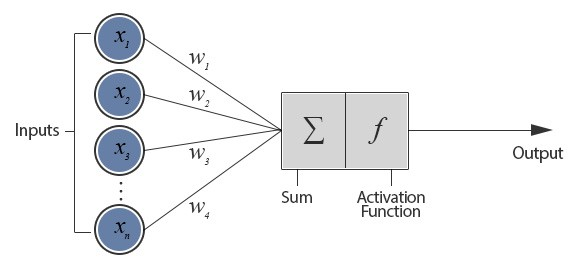
\includegraphics{neuron.jpeg}
\caption{Model of an artificial neuron.}
\end{figure}

A neuron consists of weights (\(w_i\)) and real (\(x_i\)) numbers. All
inputs injected into neurons are individually weighted, added together
and passed into the activation function. There are many different types
of activation function but one of the simplest would be step function
(another is the sigmoid).

\begin{figure}
  \begin{subfigure}{0.5\textwidth}
    \centering
    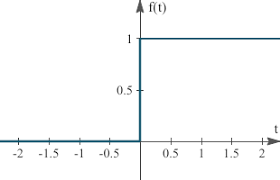
\includegraphics[width=0.9\linewidth]{step_function.png}
  \end{subfigure}
  \begin{subfigure}{0.5\textwidth}
    \centering
    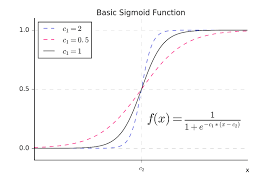
\includegraphics[width=0.9\linewidth]{sigmoid.png}
  \end{subfigure}
  \caption{Step (left) and sigmoid (right) function.}
\end{figure}
The activation function is then responsible to provide the neuron
output.

\hypertarget{training-of-a-neuron}{%
\subsubsection{Training of a neuron}\label{training-of-a-neuron}}

When teaching children how to recognize a bus, we just tell them,
showing an example: ``This is a bus. That is not a bus.'' until they
learn the concept of what a bus is. Furthermore, if the child sees new
objects that she hasn't seen before, we could expect her to recognize
correctly whether the new object is a bus or not. This is exactly the
idea behind the neurons. Similarly, inputs from a \emph{training} set
are presented to the neuron one after the other and weights are modified
according to the expected output.

When an entire pass through all of the input training vectors is
completed the neuron has learnt ! At this time, if an input vector
$\vec{P}$ (already in the training set) is given to the neuron, it
will output the correct value. If $\vec{P}$ is not in the training
set, the network will respond with an output similar to other training
vectors close to $\vec{P}$.

Unfortunately using just a neuron is not too useful since it is not
possible to solve the interesting problems we would like to face with
just that simple architecture. The next step is then to put together
more neurons in \emph{layers}.

\hypertarget{multi-layered-neural-networks}{%
\subsubsection{Multi-layered neural
networks}\label{multi-layered-neural-networks}}

\begin{figure}
\centering
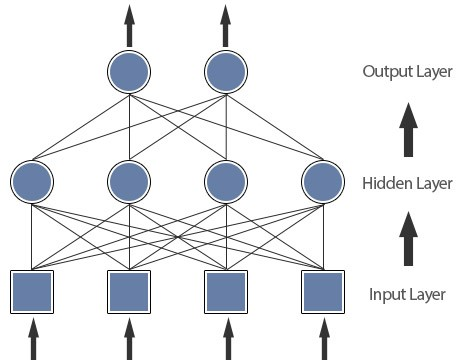
\includegraphics[width=0.7\linewidth]{multilayer.jpeg}
\caption{A multi-layered neural network.}
\end{figure}

Each input from the \emph{input layer} is fed up to each node in the
hidden layer, and from there to each node on the output layer. We should
note that there can be any number of nodes per layer and there are
usually multiple hidden layers to pass through before ultimately
reaching the output layer. But to train this network we need a learning
algorithm which should be able to tune not only the weights between the
output layer and the hidden layer but also the weights between the
hidden layer and the input layer.

\hypertarget{back-propagation}{%
\subsubsection{Back propagation}\label{back-propagation}}

First of all, we need to understand what do we lack. To tune the weights
between the hidden layer and the input layer, we need to know the error
at the hidden layer, but we know the error only at the output layer (we
know the correct output from the training sample and we also know the
output predicted by the network.) So, the method that was suggested was
to take the errors at the output layer and proportionally propagate them
backwards to the hidden layer.

So, what we are doing is:

\begin{itemize}
\tightlist
\item
  we present a training sample to the neural network (initialized with
  random weights);
\item
  compute the output received by calculating activations of each layer
  and thus calculate the error;
\item
  having calculated the error, we readjust the weights such that the
  error decreases;
\item
  we continue the process for all training samples several times until
  the weights are not changing too much.
\end{itemize}

The error is computed by the \emph{loss function} and an \emph{optimization function}
is then used to choose the appropriate weight values which reduce the loss function
(we will use \emph{Adam} as optimizator in the following but there are more).

\subsubsection{Neural Network Design}

There is no rule to guide us into the design of a neural network in terms
of number of layers and neuron per layer. The most common strategy is a
trail and error one where you finally pick up the solution giving the best accuracy.

A common mistake to avoid is to start with a too complex
(with many layers and neurons) network which usually leads to \emph{overtraining}.
Overtraining is what happens when the NN learns too well the training sample
but its performance degrade substantially in an independent testing sample.

A NN with just one hidden layer with a number of neurons averaging the inputs
and outputs is sufficient in most cases. In the following we will use more
complex networks just for illustration, no attempt in optimizing the layout has been done.

\hypertarget{neural-net-to-recognize-handwritten-digits}{%
\subsection{Neural net to recognize handwritten
digits}\label{neural-net-to-recognize-handwritten-digits}}

We don't usually appreciate how tough a problem our visual system solve
(consider that it involves 5 visual cortices containing 140 million
neurons each), but the difficulties of visual pattern recognition become
apparent if you attempt to write a computer program to recognize digits
like those below.

\begin{figure}
\centering
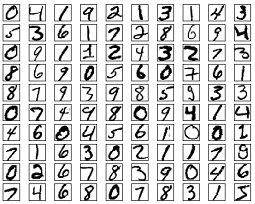
\includegraphics{mnist_100_digits.png}
\caption{The so-called MNIST training sample}
\end{figure}

Simple intuition about how we recognize shapes - ``a 9 has a loop at the
top, and a vertical stroke in the bottom right'' - turn out to be not so
simple to express algorithmically. When you try to make such rules
precise, you quickly get lost in a morass of exceptions and caveats and
special cases so that it seems hopeless.

Neural networks approach the problem in a different way. The idea is to
take a large number of handwritten digits and then develop a system
which can learn from those training examples. By increasing the number
of training examples, the network can learn more about handwriting, and
so improve its accuracy. So while I've shown just 100 training digits
above, we could certainly build a better handwriting recognizer by using
thousands or even millions or billions of training examples
(\textbf{remember that neural nets are not so capable of extrapolating
results, hence it won't recongnize a digit written in some strange way
not included in the training sample !!!}).

Let's try to implement an ANN that is capable of recognizing handwritten
digits. To start we need to install three new modules, the easiest way
of doing that is to run Anaconda on you computers (repl.it is too slow
in this case):

\begin{itemize}
\tightlist
\item
  open an anaconda-shell and type the following:
  \texttt{pip\ install\ keras,\ mnist,\ tensorflow}
\end{itemize}

\texttt{pip} is a very useful tool that allows to install new modules to
your python libraries. Alternatively using the Anaconda GUI you should be
able to install the packages using the \emph{Environment} tab.

Our program will be based on a Convolutional Neural Network (CNN, will
see later other two types of NN) which is designed for image/pattern
recognition. It works essentially by applying on top of an image a
series of filters (matrices) that works as edge detectors and with them
it classifies the images according to their features.

\begin{figure}
  \centering
  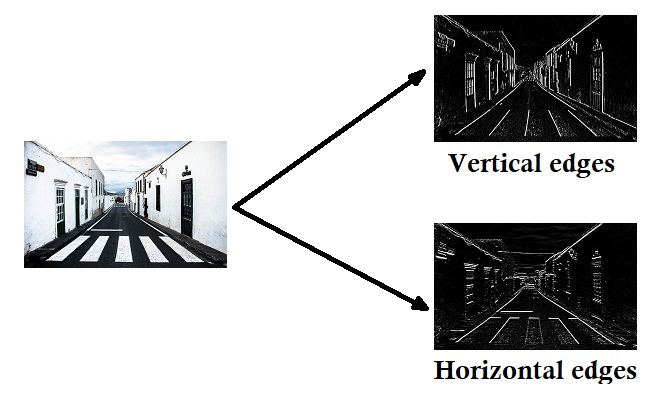
\includegraphics{edges.jpg}
  \caption{Filter application results on an image.}
\end{figure}

    \begin{tcolorbox}[breakable, size=fbox, boxrule=1pt, pad at break*=1mm,colback=cellbackground, colframe=cellborder]
\prompt{In}{incolor}{5}{\boxspacing}
\begin{Verbatim}[commandchars=\\\{\}]
\PY{k+kn}{import} \PY{n+nn}{numpy} \PY{k}{as} \PY{n+nn}{np}
\PY{c+c1}{\PYZsh{} contains our dataset for training}
\PY{k+kn}{import} \PY{n+nn}{mnist} 
\PY{c+c1}{\PYZsh{} keras gives us all the tools to work with NN}
\PY{k+kn}{from} \PY{n+nn}{keras}\PY{n+nn}{.}\PY{n+nn}{models} \PY{k}{import} \PY{n}{Sequential} 
\PY{k+kn}{from} \PY{n+nn}{keras}\PY{n+nn}{.}\PY{n+nn}{layers} \PY{k}{import} \PY{n}{Conv2D}\PY{p}{,} \PY{n}{MaxPooling2D}\PY{p}{,} \PY{n}{Dense}\PY{p}{,} \PY{n}{Flatten}
\PY{k+kn}{from} \PY{n+nn}{keras}\PY{n+nn}{.}\PY{n+nn}{utils} \PY{k}{import} \PY{n}{to\PYZus{}categorical}

\PY{c+c1}{\PYZsh{} load the training}
\PY{n}{train\PYZus{}images} \PY{o}{=} \PY{n}{mnist}\PY{o}{.}\PY{n}{train\PYZus{}images}\PY{p}{(}\PY{p}{)} \PY{c+c1}{\PYZsh{} the actual images}
\PY{n}{train\PYZus{}labels} \PY{o}{=} \PY{n}{mnist}\PY{o}{.}\PY{n}{train\PYZus{}labels}\PY{p}{(}\PY{p}{)} \PY{c+c1}{\PYZsh{} the truth (it is a 0, 1, 2...)}

\PY{c+c1}{\PYZsh{} transform data for convenience}
\PY{c+c1}{\PYZsh{}train\PYZus{}images = (train\PYZus{}images / 255) \PYZhy{} 0.5}
\PY{c+c1}{\PYZsh{} for technical reasons you need to expand axis}
\PY{n}{train\PYZus{}images} \PY{o}{=} \PY{n}{np}\PY{o}{.}\PY{n}{expand\PYZus{}dims}\PY{p}{(}\PY{n}{train\PYZus{}images}\PY{p}{,} \PY{n}{axis}\PY{o}{=}\PY{l+m+mi}{3}\PY{p}{)}

\PY{c+c1}{\PYZsh{} definition of the actual network}
\PY{n}{num\PYZus{}filters} \PY{o}{=} \PY{l+m+mi}{8}
\PY{n}{filter\PYZus{}size} \PY{o}{=} \PY{l+m+mi}{3}
\PY{n}{pool\PYZus{}size} \PY{o}{=} \PY{l+m+mi}{2}

\PY{c+c1}{\PYZsh{} the input size reflects the size of the image with}
\PY{c+c1}{\PYZsh{} the numbers 28x28 pixels}
\PY{n}{model} \PY{o}{=} \PY{n}{Sequential}\PY{p}{(}\PY{p}{[}
    \PY{n}{Conv2D}\PY{p}{(}\PY{n}{num\PYZus{}filters}\PY{p}{,} \PY{n}{filter\PYZus{}size}\PY{p}{,} \PY{n}{input\PYZus{}shape}\PY{o}{=}\PY{p}{(}\PY{l+m+mi}{28}\PY{p}{,} \PY{l+m+mi}{28}\PY{p}{,} \PY{l+m+mi}{1}\PY{p}{)}\PY{p}{)}\PY{p}{,} 
    \PY{n}{MaxPooling2D}\PY{p}{(}\PY{n}{pool\PYZus{}size}\PY{o}{=}\PY{n}{pool\PYZus{}size}\PY{p}{)}\PY{p}{,} \PY{c+c1}{\PYZsh{} reduce the size of the representation}
                                       \PY{c+c1}{\PYZsh{} to reduce the size of the parameters}
    \PY{n}{Flatten}\PY{p}{(}\PY{p}{)}\PY{p}{,} \PY{c+c1}{\PYZsh{} this step of flattening is necessary to transform a }
               \PY{c+c1}{\PYZsh{} 2D matrix into a vector to connect to a classifier}
    \PY{n}{Dense}\PY{p}{(}\PY{l+m+mi}{10}\PY{p}{,} \PY{n}{activation}\PY{o}{=}\PY{l+s+s2}{\PYZdq{}}\PY{l+s+s2}{softmax}\PY{l+s+s2}{\PYZdq{}}\PY{p}{)} \PY{c+c1}{\PYZsh{} softmax is just another type of}
                                    \PY{c+c1}{\PYZsh{} activation functions like sigmoid or step func.}
\PY{p}{]}\PY{p}{)}
\PY{c+c1}{\PYZsh{} the output is given by 10 neurons returning the }
\PY{c+c1}{\PYZsh{} probability that image is in each class.}

\PY{c+c1}{\PYZsh{} adam is an algorithm to adjust the weights every cycle}
\PY{c+c1}{\PYZsh{} loss function compute the error between the prediction and the truth }
\PY{c+c1}{\PYZsh{} metrics which error to use }
\PY{n}{model}\PY{o}{.}\PY{n}{compile}\PY{p}{(}\PY{l+s+s1}{\PYZsq{}}\PY{l+s+s1}{adam}\PY{l+s+s1}{\PYZsq{}}\PY{p}{,} \PY{n}{loss}\PY{o}{=}\PY{l+s+s2}{\PYZdq{}}\PY{l+s+s2}{categorical\PYZus{}crossentropy}\PY{l+s+s2}{\PYZdq{}}\PY{p}{,}
              \PY{n}{metrics}\PY{o}{=}\PY{p}{[}\PY{l+s+s1}{\PYZsq{}}\PY{l+s+s1}{mean\PYZus{}squared\PYZus{}error}\PY{l+s+s1}{\PYZsq{}}\PY{p}{]}\PY{p}{)}

\PY{n}{model}\PY{o}{.}\PY{n}{fit}\PY{p}{(}\PY{n}{train\PYZus{}images}\PY{p}{,}
          \PY{n}{to\PYZus{}categorical}\PY{p}{(}\PY{n}{train\PYZus{}labels}\PY{p}{)}\PY{p}{,}
          \PY{n}{epochs}\PY{o}{=}\PY{l+m+mi}{3}\PY{p}{)}\PY{c+c1}{\PYZsh{},}
          \PY{c+c1}{\PYZsh{}validation\PYZus{}data=(test\PYZus{}images, to\PYZus{}categorical(test\PYZus{}labels)))}
    
\PY{n}{model}\PY{o}{.}\PY{n}{save}\PY{p}{(}\PY{l+s+s1}{\PYZsq{}}\PY{l+s+s1}{digit\PYZus{}training.h5}\PY{l+s+s1}{\PYZsq{}}\PY{p}{)}
\end{Verbatim}
\end{tcolorbox}

    \begin{Verbatim}[commandchars=\\\{\}]
Epoch 1/3
60000/60000 [==============================] - 9s 149us/step - loss: 1.8699 -
mean\_squared\_error: 0.0193
Epoch 2/3
60000/60000 [==============================] - 9s 155us/step - loss: 0.3434 -
mean\_squared\_error: 0.0092
Epoch 3/3
60000/60000 [==============================] - 9s 148us/step - loss: 0.2325 -
mean\_squared\_error: 0.0079
    \end{Verbatim}

    Let's try to see how well our NN predicts MNIST testing digits.

    \begin{tcolorbox}[breakable, size=fbox, boxrule=1pt, pad at break*=1mm,colback=cellbackground, colframe=cellborder]
\prompt{In}{incolor}{5}{\boxspacing}
\begin{Verbatim}[commandchars=\\\{\}]
\PY{k+kn}{import} \PY{n+nn}{numpy} \PY{k}{as} \PY{n+nn}{np}
\PY{k+kn}{import} \PY{n+nn}{mnist}
\PY{k+kn}{from} \PY{n+nn}{keras}\PY{n+nn}{.}\PY{n+nn}{models} \PY{k}{import} \PY{n}{load\PYZus{}model}

\PY{n}{model} \PY{o}{=} \PY{n}{load\PYZus{}model}\PY{p}{(}\PY{l+s+s1}{\PYZsq{}}\PY{l+s+s1}{digit\PYZus{}training.h5}\PY{l+s+s1}{\PYZsq{}}\PY{p}{)}

\PY{c+c1}{\PYZsh{} testing with mnist test sample}
\PY{n}{test\PYZus{}images} \PY{o}{=} \PY{n}{mnist}\PY{o}{.}\PY{n}{test\PYZus{}images}\PY{p}{(}\PY{p}{)}
\PY{n}{test\PYZus{}labels} \PY{o}{=} \PY{n}{mnist}\PY{o}{.}\PY{n}{test\PYZus{}labels}\PY{p}{(}\PY{p}{)}

\PY{n}{test\PYZus{}images} \PY{o}{=} \PY{n}{np}\PY{o}{.}\PY{n}{expand\PYZus{}dims}\PY{p}{(}\PY{n}{test\PYZus{}images}\PY{p}{,} \PY{n}{axis}\PY{o}{=}\PY{l+m+mi}{3}\PY{p}{)}

\PY{n}{predictions} \PY{o}{=} \PY{n}{model}\PY{o}{.}\PY{n}{predict}\PY{p}{(}\PY{n}{test\PYZus{}images}\PY{p}{[}\PY{p}{:}\PY{l+m+mi}{5}\PY{p}{]}\PY{p}{)}
\PY{n+nb}{print} \PY{p}{(}\PY{l+s+s2}{\PYZdq{}}\PY{l+s+s2}{Tesing on MNIST digits...}\PY{l+s+s2}{\PYZdq{}}\PY{p}{)}
\PY{n+nb}{print}\PY{p}{(}\PY{l+s+s2}{\PYZdq{}}\PY{l+s+s2}{Predicted: }\PY{l+s+s2}{\PYZdq{}}\PY{p}{,} \PY{n}{np}\PY{o}{.}\PY{n}{argmax}\PY{p}{(}\PY{n}{predictions}\PY{p}{,} \PY{n}{axis}\PY{o}{=}\PY{l+m+mi}{1}\PY{p}{)}\PY{p}{)} 
\PY{n+nb}{print}\PY{p}{(}\PY{l+s+s2}{\PYZdq{}}\PY{l+s+s2}{Truth:}\PY{l+s+s2}{\PYZdq{}}\PY{p}{,} \PY{n}{test\PYZus{}labels}\PY{p}{[}\PY{p}{:}\PY{l+m+mi}{5}\PY{p}{]}\PY{p}{)}
\PY{n+nb}{print}\PY{p}{(}\PY{l+s+s2}{\PYZdq{}}\PY{l+s+s2}{\PYZpc{}}\PY{l+s+s2}{:}\PY{l+s+s2}{\PYZdq{}}\PY{p}{,} \PY{p}{[}\PY{l+s+s2}{\PYZdq{}}\PY{l+s+si}{\PYZob{}:.3f\PYZcb{}}\PY{l+s+s2}{\PYZdq{}}\PY{o}{.}\PY{n}{format}\PY{p}{(}\PY{n}{p}\PY{p}{[}\PY{n}{np}\PY{o}{.}\PY{n}{argmax}\PY{p}{(}\PY{n}{p}\PY{p}{)}\PY{p}{]}\PY{p}{)} \PY{k}{for} \PY{n}{p} \PY{o+ow}{in} \PY{n}{predictions}\PY{p}{]}\PY{p}{)}
\end{Verbatim}
\end{tcolorbox}

    \begin{Verbatim}[commandchars=\\\{\}]
Tesing on MNIST digits{\ldots}
Predicted:  [7 2 1 0 4]
Truth: [7 2 1 0 4]
\%: ['1.000', '1.000', '0.995', '1.000', '1.000']
    \end{Verbatim}

    To see how well our NN behaves with different kind of digits we will try
to check how it works with your own calligraphy.

\begin{itemize}
\tightlist
\item
  Open \texttt{paint} and create a 280x280 white square
\item
  Change brush type and set the maximum size
\item
  With the mouse draw a digit
\item
  Finally save the file (e.g.~five.png)
\end{itemize}

Before passing the image to the NN it has to be resized and this is done
with an ad hoc function (\texttt{transform\_image}).

    \begin{tcolorbox}[breakable, size=fbox, boxrule=1pt, pad at break*=1mm,colback=cellbackground, colframe=cellborder]
\prompt{In}{incolor}{6}{\boxspacing}
\begin{Verbatim}[commandchars=\\\{\}]
\PY{k+kn}{import} \PY{n+nn}{numpy} \PY{k}{as} \PY{n+nn}{np}
\PY{k+kn}{from} \PY{n+nn}{keras}\PY{n+nn}{.}\PY{n+nn}{models} \PY{k}{import} \PY{n}{load\PYZus{}model}
\PY{k+kn}{from} \PY{n+nn}{digit\PYZus{}converter} \PY{k}{import} \PY{n}{transform\PYZus{}image}

\PY{n}{model} \PY{o}{=} \PY{n}{load\PYZus{}model}\PY{p}{(}\PY{l+s+s1}{\PYZsq{}}\PY{l+s+s1}{digit\PYZus{}training.h5}\PY{l+s+s1}{\PYZsq{}}\PY{p}{)}

\PY{n}{test\PYZus{}images} \PY{o}{=} \PY{n}{np}\PY{o}{.}\PY{n}{array}\PY{p}{(}\PY{n}{transform\PYZus{}image}\PY{p}{(}\PY{l+s+s2}{\PYZdq{}}\PY{l+s+s2}{five.png}\PY{l+s+s2}{\PYZdq{}}\PY{p}{)}\PY{p}{)}
\PY{n}{test\PYZus{}images} \PY{o}{=} \PY{n}{np}\PY{o}{.}\PY{n}{expand\PYZus{}dims}\PY{p}{(}\PY{n}{test\PYZus{}images}\PY{p}{,} \PY{n}{axis}\PY{o}{=}\PY{l+m+mi}{3}\PY{p}{)}

\PY{n}{predict} \PY{o}{=} \PY{n}{model}\PY{o}{.}\PY{n}{predict}\PY{p}{(}\PY{n}{test\PYZus{}images}\PY{p}{)}
\PY{n+nb}{print} \PY{p}{(}\PY{l+s+s2}{\PYZdq{}}\PY{l+s+se}{\PYZbs{}n}\PY{l+s+s2}{\PYZdq{}}\PY{p}{)}
\PY{n+nb}{print} \PY{p}{(}\PY{l+s+s2}{\PYZdq{}}\PY{l+s+s2}{Tesing on custom digits...}\PY{l+s+s2}{\PYZdq{}}\PY{p}{)}
\PY{n+nb}{print} \PY{p}{(}\PY{l+s+s2}{\PYZdq{}}\PY{l+s+s2}{Predicted: }\PY{l+s+s2}{\PYZdq{}}\PY{p}{,} \PY{n}{np}\PY{o}{.}\PY{n}{argmax}\PY{p}{(}\PY{n}{predict}\PY{p}{,} \PY{n}{axis}\PY{o}{=}\PY{l+m+mi}{1}\PY{p}{)}\PY{p}{)}
\PY{n+nb}{print}\PY{p}{(}\PY{l+s+s2}{\PYZdq{}}\PY{l+s+s2}{\PYZpc{}}\PY{l+s+s2}{:}\PY{l+s+s2}{\PYZdq{}}\PY{p}{,} \PY{p}{[}\PY{l+s+s2}{\PYZdq{}}\PY{l+s+si}{\PYZob{}:.3f\PYZcb{}}\PY{l+s+s2}{\PYZdq{}}\PY{o}{.}\PY{n}{format}\PY{p}{(}\PY{n}{p}\PY{p}{[}\PY{n}{np}\PY{o}{.}\PY{n}{argmax}\PY{p}{(}\PY{n}{p}\PY{p}{)}\PY{p}{]}\PY{p}{)} \PY{k}{for} \PY{n}{p} \PY{o+ow}{in} \PY{n}{predict}\PY{p}{]}\PY{p}{)}
\end{Verbatim}
\end{tcolorbox}

    \begin{Verbatim}[commandchars=\\\{\}]


Tesing on custom digits{\ldots}
Predicted:  [5]
\%: ['0.739']
    \end{Verbatim}

    Those the images I have checked:
    \begin{center}
    
\includegraphics[width=0.2\linewidth]{four.png}
    
\includegraphics[width=0.2\linewidth]{five.png}
    \end{center}
    
    \hypertarget{black-scholes-call-options}{%
\subsection{Black-Scholes call
options}\label{black-scholes-call-options}}

The first financial application of a NN concerns the pricing of european
call options. In this case I have generated myself a large number of
call options with a strike (100) and a maturity (1 year), simulated the
underlying development and finally trained the NN using as inputs:
volatility, strike, maturity and the underlying. The truth is the price
of the call computed using the Black-Scholes formula.

\begin{figure}
  \centering
  
\includegraphics{underlyings.png}
  \caption{Some of the underlying development used in the BS simulation.}
\end{figure}

The code used for the simulation is in
\(\href{https://repl.it/@MatteoSani/exercises8}{\textrm{bs\_simulation.py}}\).
I have also simulated two testing samples, one with the parameters
included in the training events, and one with parameters outside. The
training and testing samples have been stored in a \emph{csv}
(comma-separated values) file, which has a particular format very easy
to read.

In the training I have used a \emph{traditional} NN with an input layer
with 4 neurons (the number of inputs), an hidden layer with 10 neurons
and an output layer with 1 single neuron (since I need just a number,
the price of the call).

    \begin{tcolorbox}[breakable, size=fbox, boxrule=1pt, pad at break*=1mm,colback=cellbackground, colframe=cellborder]
\prompt{In}{incolor}{7}{\boxspacing}
\begin{Verbatim}[commandchars=\\\{\}]
\PY{c+c1}{\PYZsh{} Regression Example }
\PY{k+kn}{from} \PY{n+nn}{keras}\PY{n+nn}{.}\PY{n+nn}{models} \PY{k}{import} \PY{n}{Sequential}\PY{p}{,} \PY{n}{load\PYZus{}model}
\PY{k+kn}{from} \PY{n+nn}{keras}\PY{n+nn}{.}\PY{n+nn}{layers} \PY{k}{import} \PY{n}{Dense}
\PY{k+kn}{import} \PY{n+nn}{pandas} \PY{k}{as} \PY{n+nn}{pd}

\PY{n}{dataset} \PY{o}{=} \PY{n}{pd}\PY{o}{.}\PY{n}{read\PYZus{}csv}\PY{p}{(}\PY{l+s+s2}{\PYZdq{}}\PY{l+s+s2}{bs\PYZus{}training.csv}\PY{l+s+s2}{\PYZdq{}}\PY{p}{)}
\PY{n}{X\PYZus{}train} \PY{o}{=} \PY{n}{dataset}\PY{o}{.}\PY{n}{iloc}\PY{p}{[}\PY{p}{:}\PY{p}{,} \PY{p}{:}\PY{l+m+mi}{4}\PY{p}{]}\PY{o}{.}\PY{n}{values}
\PY{n}{Y\PYZus{}train} \PY{o}{=} \PY{n}{dataset}\PY{o}{.}\PY{n}{iloc}\PY{p}{[}\PY{p}{:}\PY{p}{,} \PY{l+m+mi}{4}\PY{p}{]}\PY{o}{.}\PY{n}{values}

\PY{c+c1}{\PYZsh{} create model}
\PY{n}{model} \PY{o}{=} \PY{n}{Sequential}\PY{p}{(}\PY{p}{)}
\PY{n}{model}\PY{o}{.}\PY{n}{add}\PY{p}{(}\PY{n}{Dense}\PY{p}{(}\PY{l+m+mi}{15}\PY{p}{,} \PY{n}{input\PYZus{}dim}\PY{o}{=}\PY{l+m+mi}{4}\PY{p}{,} \PY{n}{kernel\PYZus{}initializer}\PY{o}{=}\PY{l+s+s1}{\PYZsq{}}\PY{l+s+s1}{normal}\PY{l+s+s1}{\PYZsq{}}\PY{p}{,} \PY{n}{activation}\PY{o}{=}\PY{l+s+s1}{\PYZsq{}}\PY{l+s+s1}{relu}\PY{l+s+s1}{\PYZsq{}}\PY{p}{)}\PY{p}{)}
\PY{n}{model}\PY{o}{.}\PY{n}{add}\PY{p}{(}\PY{n}{Dense}\PY{p}{(}\PY{l+m+mi}{10}\PY{p}{,} \PY{n}{kernel\PYZus{}initializer}\PY{o}{=}\PY{l+s+s1}{\PYZsq{}}\PY{l+s+s1}{normal}\PY{l+s+s1}{\PYZsq{}}\PY{p}{,} \PY{n}{activation}\PY{o}{=}\PY{l+s+s1}{\PYZsq{}}\PY{l+s+s1}{relu}\PY{l+s+s1}{\PYZsq{}}\PY{p}{)}\PY{p}{)}
\PY{n}{model}\PY{o}{.}\PY{n}{add}\PY{p}{(}\PY{n}{Dense}\PY{p}{(}\PY{l+m+mi}{5}\PY{p}{,} \PY{n}{kernel\PYZus{}initializer}\PY{o}{=}\PY{l+s+s1}{\PYZsq{}}\PY{l+s+s1}{normal}\PY{l+s+s1}{\PYZsq{}}\PY{p}{,} \PY{n}{activation}\PY{o}{=}\PY{l+s+s1}{\PYZsq{}}\PY{l+s+s1}{relu}\PY{l+s+s1}{\PYZsq{}}\PY{p}{)}\PY{p}{)}
\PY{n}{model}\PY{o}{.}\PY{n}{add}\PY{p}{(}\PY{n}{Dense}\PY{p}{(}\PY{l+m+mi}{1}\PY{p}{,} \PY{n}{kernel\PYZus{}initializer}\PY{o}{=}\PY{l+s+s1}{\PYZsq{}}\PY{l+s+s1}{normal}\PY{l+s+s1}{\PYZsq{}}\PY{p}{)}\PY{p}{)}

\PY{n}{model}\PY{o}{.}\PY{n}{compile}\PY{p}{(}\PY{n}{loss}\PY{o}{=}\PY{l+s+s1}{\PYZsq{}}\PY{l+s+s1}{mean\PYZus{}absolute\PYZus{}error}\PY{l+s+s1}{\PYZsq{}}\PY{p}{,} \PY{n}{optimizer}\PY{o}{=}\PY{l+s+s1}{\PYZsq{}}\PY{l+s+s1}{adam}\PY{l+s+s1}{\PYZsq{}}\PY{p}{,} \PY{n}{metrics}\PY{o}{=}\PY{p}{[}\PY{l+s+s1}{\PYZsq{}}\PY{l+s+s1}{mse}\PY{l+s+s1}{\PYZsq{}}\PY{p}{,} \PY{l+s+s1}{\PYZsq{}}\PY{l+s+s1}{mae}\PY{l+s+s1}{\PYZsq{}}\PY{p}{]}\PY{p}{)}

\PY{n}{history} \PY{o}{=} \PY{n}{model}\PY{o}{.}\PY{n}{fit}\PY{p}{(}\PY{n}{X\PYZus{}train}\PY{p}{,} \PY{n}{Y\PYZus{}train}\PY{p}{,} \PY{n}{epochs}\PY{o}{=}\PY{l+m+mi}{1000}\PY{p}{,} \PY{n}{verbose}\PY{o}{=}\PY{l+m+mi}{1}\PY{p}{)}\PY{c+c1}{\PYZsh{}, batch\PYZus{}size=10)}
\PY{n}{evaluator} \PY{o}{=} \PY{n}{model}\PY{o}{.}\PY{n}{evaluate}\PY{p}{(}\PY{n}{X\PYZus{}train}\PY{p}{,} \PY{n}{Y\PYZus{}train}\PY{p}{)}
\PY{n+nb}{print}\PY{p}{(}\PY{l+s+s1}{\PYZsq{}}\PY{l+s+s1}{Test: }\PY{l+s+si}{\PYZob{}\PYZcb{}}\PY{l+s+s1}{\PYZsq{}}\PY{o}{.}\PY{n}{format}\PY{p}{(}\PY{n}{evaluator}\PY{p}{)}\PY{p}{)}

\PY{n}{model}\PY{o}{.}\PY{n}{save}\PY{p}{(}\PY{l+s+s1}{\PYZsq{}}\PY{l+s+s1}{bs\PYZus{}model.h5}\PY{l+s+s1}{\PYZsq{}}\PY{p}{)}
\end{Verbatim}
\end{tcolorbox}

    \begin{Verbatim}[commandchars=\\\{\}]
Epoch 1/1000
2919/2919 [==============================] - 0s 90us/step - loss: 12.5533 - mse:
258.4865 - mae: 12.5533
...
Epoch 50/1000
2919/2919 [==============================] - 0s 49us/step - loss: 2.4020 - mse:
8.7222 - mae: 2.4020
...
Epoch 1000/1000
2919/2919 [==============================] - 0s 35us/step - loss: 0.1038 - mse:
0.0183 - mae: 0.1038
2919/2919 [==============================] - 0s 33us/step
Test: [0.08122403969150388, 0.011596422642469406, 0.08122401684522629]
    \end{Verbatim}

    Let's see now how the NN behaves with the two testing samples. First the
one generated with parameters in the training phase space.

    \begin{tcolorbox}[breakable, size=fbox, boxrule=1pt, pad at break*=1mm,colback=cellbackground, colframe=cellborder]
\prompt{In}{incolor}{9}{\boxspacing}
\begin{Verbatim}[commandchars=\\\{\}]
\PY{k+kn}{from} \PY{n+nn}{keras}\PY{n+nn}{.}\PY{n+nn}{models} \PY{k}{import} \PY{n}{load\PYZus{}model}
\PY{k+kn}{import} \PY{n+nn}{pandas} \PY{k}{as} \PY{n+nn}{pd}
\PY{k+kn}{import} \PY{n+nn}{matplotlib}\PY{n+nn}{.}\PY{n+nn}{pyplot} \PY{k}{as} \PY{n+nn}{plt}

\PY{n}{model} \PY{o}{=} \PY{n}{load\PYZus{}model}\PY{p}{(}\PY{l+s+s1}{\PYZsq{}}\PY{l+s+s1}{bs\PYZus{}model.h5}\PY{l+s+s1}{\PYZsq{}}\PY{p}{)}

\PY{n}{dataset} \PY{o}{=} \PY{n}{pd}\PY{o}{.}\PY{n}{read\PYZus{}csv}\PY{p}{(}\PY{l+s+s2}{\PYZdq{}}\PY{l+s+s2}{bs\PYZus{}testing.csv}\PY{l+s+s2}{\PYZdq{}}\PY{p}{)}
\PY{n}{X\PYZus{}test} \PY{o}{=} \PY{n}{dataset}\PY{o}{.}\PY{n}{iloc}\PY{p}{[}\PY{p}{:}\PY{p}{,} \PY{p}{:}\PY{l+m+mi}{4}\PY{p}{]}\PY{o}{.}\PY{n}{values}
\PY{n}{Y\PYZus{}test} \PY{o}{=} \PY{n}{dataset}\PY{o}{.}\PY{n}{iloc}\PY{p}{[}\PY{p}{:}\PY{p}{,} \PY{l+m+mi}{4}\PY{p}{]}\PY{o}{.}\PY{n}{values}

\PY{n}{plt}\PY{o}{.}\PY{n}{plot}\PY{p}{(}\PY{n}{model}\PY{o}{.}\PY{n}{predict}\PY{p}{(}\PY{n}{X\PYZus{}test}\PY{p}{)}\PY{p}{,} \PY{n}{color}\PY{o}{=}\PY{l+s+s2}{\PYZdq{}}\PY{l+s+s2}{red}\PY{l+s+s2}{\PYZdq{}}\PY{p}{,} \PY{n}{label}\PY{o}{=}\PY{l+s+s2}{\PYZdq{}}\PY{l+s+s2}{NN price}\PY{l+s+s2}{\PYZdq{}}\PY{p}{)}
\PY{n}{plt}\PY{o}{.}\PY{n}{plot}\PY{p}{(}\PY{n}{Y\PYZus{}test}\PY{p}{,} \PY{n}{label}\PY{o}{=}\PY{l+s+s2}{\PYZdq{}}\PY{l+s+s2}{BS price}\PY{l+s+s2}{\PYZdq{}}\PY{p}{)}
\PY{n}{plt}\PY{o}{.}\PY{n}{legend}\PY{p}{(}\PY{p}{)}
\PY{n}{plt}\PY{o}{.}\PY{n}{show}\PY{p}{(}\PY{p}{)}
\PY{n}{plt}\PY{o}{.}\PY{n}{savefig}\PY{p}{(}\PY{l+s+s2}{\PYZdq{}}\PY{l+s+s2}{comparison\PYZus{}fair.png}\PY{l+s+s2}{\PYZdq{}}\PY{p}{)}
\end{Verbatim}
\end{tcolorbox}

    \begin{figure}
      \begin{center}
        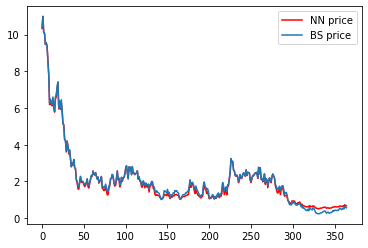
\includegraphics[width=0.8\linewidth]{lecture_8_files/lecture_8_9_0.png}
      \end{center}
      \caption{Comparison of neural network prediction (red) to BS pricing (blue).}
    \end{figure}
    
    The agreement is pretty good. To illustrate how a neural network is not
able to extrapolate results if the prediction is tried with inputs
outside the phase-space of the training (i.e.~testing sample different
from the one used in the training) I have tried to predict the price of
a call with different maturity (strike and vol are in the range of the
training instead):

    \begin{tcolorbox}[breakable, size=fbox, boxrule=1pt, pad at break*=1mm,colback=cellbackground, colframe=cellborder]
\prompt{In}{incolor}{10}{\boxspacing}
\begin{Verbatim}[commandchars=\\\{\}]
\PY{k+kn}{from} \PY{n+nn}{keras}\PY{n+nn}{.}\PY{n+nn}{models} \PY{k}{import} \PY{n}{load\PYZus{}model}
\PY{k+kn}{import} \PY{n+nn}{pandas} \PY{k}{as} \PY{n+nn}{pd}
\PY{k+kn}{import} \PY{n+nn}{matplotlib}\PY{n+nn}{.}\PY{n+nn}{pyplot} \PY{k}{as} \PY{n+nn}{plt}

\PY{n}{model} \PY{o}{=} \PY{n}{load\PYZus{}model}\PY{p}{(}\PY{l+s+s1}{\PYZsq{}}\PY{l+s+s1}{bs\PYZus{}model.h5}\PY{l+s+s1}{\PYZsq{}}\PY{p}{)}

\PY{n}{dataset} \PY{o}{=} \PY{n}{pd}\PY{o}{.}\PY{n}{read\PYZus{}csv}\PY{p}{(}\PY{l+s+s2}{\PYZdq{}}\PY{l+s+s2}{bs\PYZus{}testing\PYZus{}off.csv}\PY{l+s+s2}{\PYZdq{}}\PY{p}{)}
\PY{n}{X\PYZus{}test} \PY{o}{=} \PY{n}{dataset}\PY{o}{.}\PY{n}{iloc}\PY{p}{[}\PY{p}{:}\PY{p}{,} \PY{p}{:}\PY{l+m+mi}{4}\PY{p}{]}\PY{o}{.}\PY{n}{values}
\PY{n}{Y\PYZus{}test} \PY{o}{=} \PY{n}{dataset}\PY{o}{.}\PY{n}{iloc}\PY{p}{[}\PY{p}{:}\PY{p}{,} \PY{l+m+mi}{4}\PY{p}{]}\PY{o}{.}\PY{n}{values}

\PY{n}{plt}\PY{o}{.}\PY{n}{plot}\PY{p}{(}\PY{n}{model}\PY{o}{.}\PY{n}{predict}\PY{p}{(}\PY{n}{X\PYZus{}test}\PY{p}{)}\PY{p}{,} \PY{n}{color}\PY{o}{=}\PY{l+s+s2}{\PYZdq{}}\PY{l+s+s2}{red}\PY{l+s+s2}{\PYZdq{}}\PY{p}{,} \PY{n}{label}\PY{o}{=}\PY{l+s+s2}{\PYZdq{}}\PY{l+s+s2}{NN price}\PY{l+s+s2}{\PYZdq{}}\PY{p}{)}
\PY{n}{plt}\PY{o}{.}\PY{n}{plot}\PY{p}{(}\PY{n}{Y\PYZus{}test}\PY{p}{,} \PY{n}{label}\PY{o}{=}\PY{l+s+s2}{\PYZdq{}}\PY{l+s+s2}{BS price}\PY{l+s+s2}{\PYZdq{}}\PY{p}{)}
\PY{n}{plt}\PY{o}{.}\PY{n}{legend}\PY{p}{(}\PY{p}{)}
\PY{n}{plt}\PY{o}{.}\PY{n}{show}\PY{p}{(}\PY{p}{)}
\PY{n}{plt}\PY{o}{.}\PY{n}{savefig}\PY{p}{(}\PY{l+s+s2}{\PYZdq{}}\PY{l+s+s2}{comparison\PYZus{}off.png}\PY{l+s+s2}{\PYZdq{}}\PY{p}{)}
\end{Verbatim}
\end{tcolorbox}
    
    \begin{figure}
      \begin{center}
        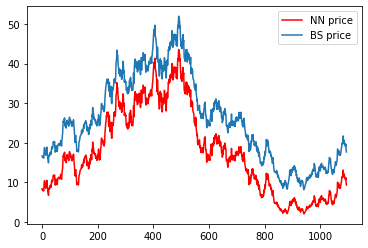
\includegraphics[width=0.8\linewidth]{lecture_8_files/lecture_8_11_0.png}
      \end{center}
      \caption{Comparison of neural network prediction (red) to BS pricing (blue) on a simulation done with
        parameter values outside the training phase-space.}
    \end{figure}

    
    \hypertarget{technical-analysis}{%
\subsection{Technical Analysis}\label{technical-analysis}}

In finance, technical analysis is a security analysis discipline for
forecasting the direction of prices through the study of past market
data, primarily price and volume. Essentially the analyst looks for
particular patterns in the price time series that are \emph{known} to
develop in predictable ways to take profit of it.

\begin{figure}
  \begin{subfigure}{.5\textwidth}
    \centering
    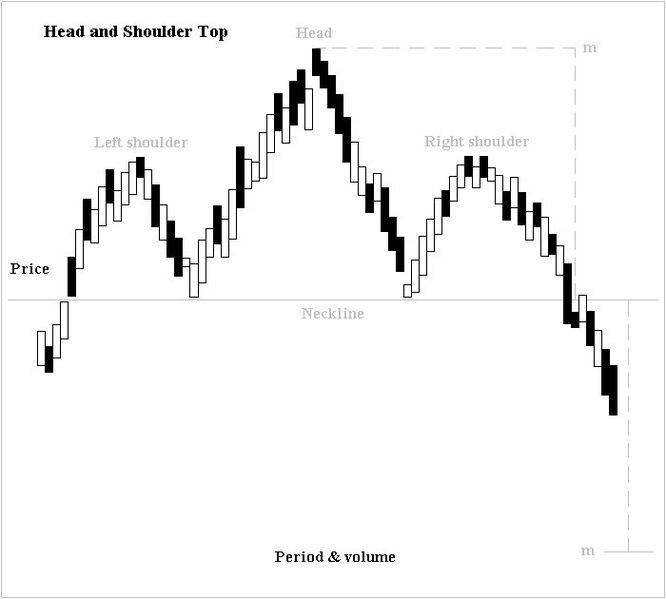
\includegraphics[width=0.8\linewidth]{H_and_s_top_new.jpg}
    \caption{Head and shoulders pattern in real data.}
  \end{subfigure}
  \begin{subfigure}{.5\textwidth}
    \centering
    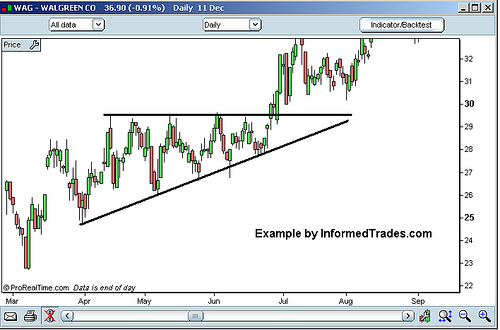
\includegraphics[width=0.8\linewidth]{Triangle-ascending.jpg}
    \caption{Ascending triangle pattern in real data.}
  \end{subfigure}
\end{figure}

As you may imagine we will try to develop a CNN (like in the handwriting
case) capable of classifying features in time series to be used in a
technical analysis (this is much faster than having somebody looking at
thousands of time series by eye\ldots{}).

As in the previous application I have generated myself the training set
simulating 21600 time series (1/3 with head and shoulder patter, 1/3
with triangle pattern and 1/3 with no pattern). \emph{To make the
training easier the features have been exagerated.}

\begin{figure}
  \begin{subfigure}{.5\textwidth}
    \centering
    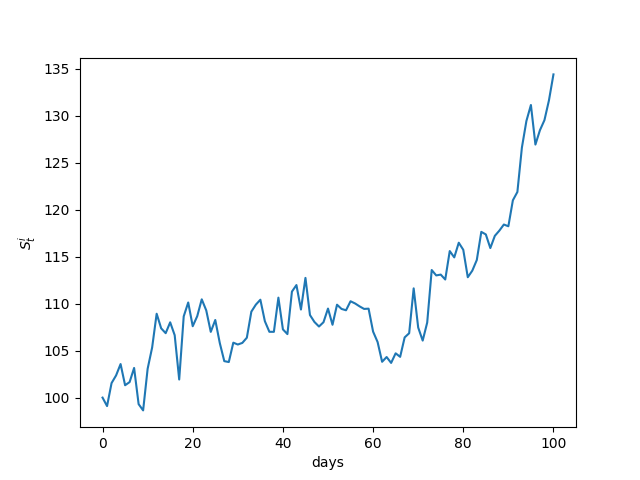
\includegraphics[width=.8\linewidth]{image_1.png}
    \caption{No pattern}
  \end{subfigure}
  \begin{subfigure}{.5\textwidth}
    \centering    
    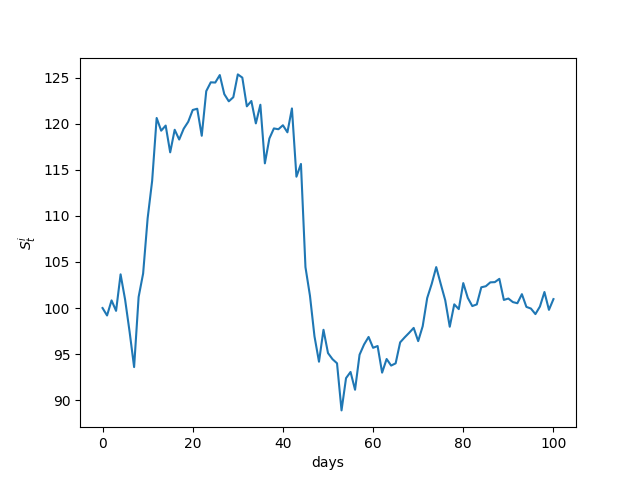
\includegraphics[width=.8\linewidth]{image_2.png}
    \caption{Head and shoulder pattern}    
  \end{subfigure}
  \begin{subfigure}{.5\textwidth}
    \centering    
    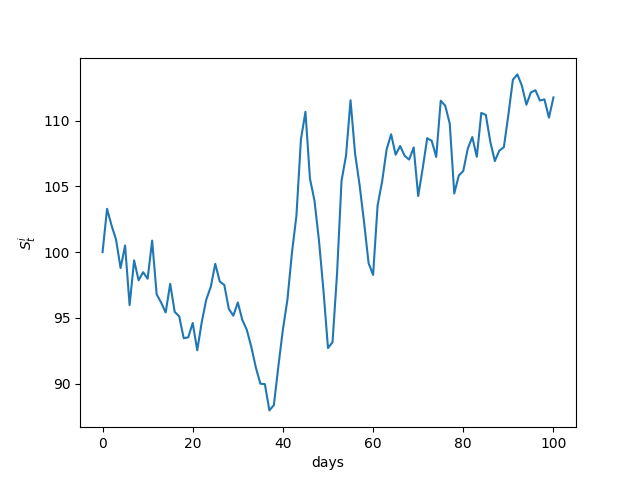
\includegraphics[width=.8\linewidth]{image_0.png}
    \caption{Tringle pattern}    
  \end{subfigure}
\end{figure}

    \begin{tcolorbox}[breakable, size=fbox, boxrule=1pt, pad at break*=1mm,colback=cellbackground, colframe=cellborder]
\prompt{In}{incolor}{20}{\boxspacing}
\begin{Verbatim}[commandchars=\\\{\}]
\PY{k+kn}{import} \PY{n+nn}{numpy} \PY{k}{as} \PY{n+nn}{np}
\PY{k+kn}{import} \PY{n+nn}{json}
\PY{k+kn}{from} \PY{n+nn}{keras}\PY{n+nn}{.}\PY{n+nn}{models} \PY{k}{import} \PY{n}{Sequential}\PY{p}{,} \PY{n}{load\PYZus{}model}
\PY{k+kn}{from} \PY{n+nn}{keras}\PY{n+nn}{.}\PY{n+nn}{layers} \PY{k}{import} \PY{n}{Dense}\PY{p}{,} \PY{n}{Conv1D}\PY{p}{,} \PY{n}{Dropout}\PY{p}{,} \PY{n}{MaxPooling1D}\PY{p}{,} \PY{n}{Flatten}\PY{p}{,} \PY{n}{GlobalAveragePooling1D}
\PY{k+kn}{from} \PY{n+nn}{keras}\PY{n+nn}{.}\PY{n+nn}{utils} \PY{k}{import} \PY{n}{to\PYZus{}categorical}

\PY{c+c1}{\PYZsh{} load the training set}
\PY{k}{with} \PY{n+nb}{open}\PY{p}{(}\PY{l+s+s2}{\PYZdq{}}\PY{l+s+s2}{training\PYZus{}techana\PYZus{}labels.json}\PY{l+s+s2}{\PYZdq{}}\PY{p}{,} \PY{l+s+s2}{\PYZdq{}}\PY{l+s+s2}{r}\PY{l+s+s2}{\PYZdq{}}\PY{p}{)} \PY{k}{as} \PY{n}{f}\PY{p}{:}
    \PY{n}{train\PYZus{}labels} \PY{o}{=} \PY{n}{json}\PY{o}{.}\PY{n}{load}\PY{p}{(}\PY{n}{f}\PY{p}{)}
\PY{n}{train\PYZus{}labels} \PY{o}{=} \PY{n}{train\PYZus{}labels}\PY{p}{[}\PY{p}{:}\PY{l+m+mi}{3000}\PY{p}{]}
\PY{n}{train\PYZus{}images} \PY{o}{=} \PY{p}{[}\PY{p}{]}

\PY{k}{with} \PY{n+nb}{open}\PY{p}{(}\PY{l+s+s2}{\PYZdq{}}\PY{l+s+s2}{training\PYZus{}techana\PYZus{}images.json}\PY{l+s+s2}{\PYZdq{}}\PY{p}{,} \PY{l+s+s2}{\PYZdq{}}\PY{l+s+s2}{r}\PY{l+s+s2}{\PYZdq{}}\PY{p}{)} \PY{k}{as} \PY{n}{f}\PY{p}{:}
    \PY{n}{train\PYZus{}images} \PY{o}{=} \PY{n}{json}\PY{o}{.}\PY{n}{load}\PY{p}{(}\PY{n}{f}\PY{p}{)}
\PY{n}{train\PYZus{}images} \PY{o}{=} \PY{n}{train\PYZus{}images}\PY{p}{[}\PY{p}{:}\PY{l+m+mi}{3000}\PY{p}{]}
\PY{n}{train\PYZus{}images} \PY{o}{=} \PY{n}{np}\PY{o}{.}\PY{n}{array}\PY{p}{(}\PY{n}{train\PYZus{}images}\PY{p}{)}
\PY{n}{train\PYZus{}images} \PY{o}{=} \PY{n}{np}\PY{o}{.}\PY{n}{expand\PYZus{}dims}\PY{p}{(}\PY{n}{train\PYZus{}images}\PY{p}{,} \PY{n}{axis}\PY{o}{=}\PY{l+m+mi}{3}\PY{p}{)}

\PY{c+c1}{\PYZsh{} define the CNN }
\PY{n}{model} \PY{o}{=} \PY{n}{Sequential}\PY{p}{(}\PY{p}{)}
\PY{n}{model}\PY{o}{.}\PY{n}{add}\PY{p}{(}\PY{n}{Conv1D}\PY{p}{(}\PY{n}{filters}\PY{o}{=}\PY{l+m+mi}{80}\PY{p}{,} \PY{n}{kernel\PYZus{}size}\PY{o}{=}\PY{l+m+mi}{20}\PY{p}{,} 
                 \PY{n}{activation}\PY{o}{=}\PY{l+s+s1}{\PYZsq{}}\PY{l+s+s1}{relu}\PY{l+s+s1}{\PYZsq{}}\PY{p}{,} \PY{n}{input\PYZus{}shape}\PY{o}{=}\PY{p}{(}\PY{l+m+mi}{101}\PY{p}{,} \PY{l+m+mi}{1}\PY{p}{)}\PY{p}{)}\PY{p}{)}
\PY{n}{model}\PY{o}{.}\PY{n}{add}\PY{p}{(}\PY{n}{Conv1D}\PY{p}{(}\PY{n}{filters}\PY{o}{=}\PY{l+m+mi}{80}\PY{p}{,} \PY{n}{kernel\PYZus{}size}\PY{o}{=}\PY{l+m+mi}{15}\PY{p}{,} 
                 \PY{n}{activation}\PY{o}{=}\PY{l+s+s1}{\PYZsq{}}\PY{l+s+s1}{relu}\PY{l+s+s1}{\PYZsq{}}\PY{p}{)}\PY{p}{)}
\PY{n}{model}\PY{o}{.}\PY{n}{add}\PY{p}{(}\PY{n}{MaxPooling1D}\PY{p}{(}\PY{l+m+mi}{3}\PY{p}{)}\PY{p}{)}
\PY{n}{model}\PY{o}{.}\PY{n}{add}\PY{p}{(}\PY{n}{Conv1D}\PY{p}{(}\PY{n}{filters}\PY{o}{=}\PY{l+m+mi}{100}\PY{p}{,} \PY{n}{kernel\PYZus{}size}\PY{o}{=}\PY{l+m+mi}{10}\PY{p}{,} 
                 \PY{n}{activation}\PY{o}{=}\PY{l+s+s1}{\PYZsq{}}\PY{l+s+s1}{relu}\PY{l+s+s1}{\PYZsq{}}\PY{p}{)}\PY{p}{)}
\PY{n}{model}\PY{o}{.}\PY{n}{add}\PY{p}{(}\PY{n}{Conv1D}\PY{p}{(}\PY{n}{filters}\PY{o}{=}\PY{l+m+mi}{100}\PY{p}{,} \PY{n}{kernel\PYZus{}size}\PY{o}{=}\PY{l+m+mi}{5}\PY{p}{,} 
                 \PY{n}{activation}\PY{o}{=}\PY{l+s+s1}{\PYZsq{}}\PY{l+s+s1}{relu}\PY{l+s+s1}{\PYZsq{}}\PY{p}{)}\PY{p}{)}
\PY{n}{model}\PY{o}{.}\PY{n}{add}\PY{p}{(}\PY{n}{GlobalAveragePooling1D}\PY{p}{(}\PY{p}{)}\PY{p}{)}
\PY{n}{model}\PY{o}{.}\PY{n}{add}\PY{p}{(}\PY{n}{Dropout}\PY{p}{(}\PY{l+m+mf}{0.5}\PY{p}{)}\PY{p}{)}
\PY{c+c1}{\PYZsh{}model.add(Flatten())}
\PY{n}{model}\PY{o}{.}\PY{n}{add}\PY{p}{(}\PY{n}{Dense}\PY{p}{(}\PY{l+m+mi}{3}\PY{p}{,} \PY{n}{activation}\PY{o}{=}\PY{l+s+s2}{\PYZdq{}}\PY{l+s+s2}{softmax}\PY{l+s+s2}{\PYZdq{}}\PY{p}{)}\PY{p}{)}
\PY{n}{model}\PY{o}{.}\PY{n}{compile}\PY{p}{(}\PY{n}{loss}\PY{o}{=}\PY{l+s+s1}{\PYZsq{}}\PY{l+s+s1}{categorical\PYZus{}crossentropy}\PY{l+s+s1}{\PYZsq{}}\PY{p}{,} 
              \PY{n}{optimizer}\PY{o}{=}\PY{l+s+s1}{\PYZsq{}}\PY{l+s+s1}{adam}\PY{l+s+s1}{\PYZsq{}}\PY{p}{,} \PY{n}{metrics}\PY{o}{=}\PY{p}{[}\PY{l+s+s1}{\PYZsq{}}\PY{l+s+s1}{accuracy}\PY{l+s+s1}{\PYZsq{}}\PY{p}{]}\PY{p}{)}

\PY{c+c1}{\PYZsh{} make the training}
\PY{n}{model}\PY{o}{.}\PY{n}{fit}\PY{p}{(}\PY{n}{train\PYZus{}images}\PY{p}{,} \PY{n}{to\PYZus{}categorical}\PY{p}{(}\PY{n}{train\PYZus{}labels}\PY{p}{)}\PY{p}{,} 
          \PY{n}{epochs}\PY{o}{=}\PY{l+m+mi}{80}\PY{p}{,} \PY{n}{batch\PYZus{}size}\PY{o}{=}\PY{l+m+mi}{35}\PY{p}{,} \PY{n}{verbose}\PY{o}{=}\PY{l+m+mi}{2}\PY{p}{)}

\PY{n}{model}\PY{o}{.}\PY{n}{save}\PY{p}{(}\PY{l+s+s1}{\PYZsq{}}\PY{l+s+s1}{techana.h5}\PY{l+s+s1}{\PYZsq{}}\PY{p}{)}
\end{Verbatim}
\end{tcolorbox}

    \begin{Verbatim}[commandchars=\\\{\}]
Epoch 1/80
 - 2s - loss: 0.9404 - accuracy: 0.7007
...
 Epoch 40/80
 - 2s - loss: 0.3310 - accuracy: 0.8697
...
 Epoch 80/80
 - 1s - loss: 0.1953 - accuracy: 0.9237
    \end{Verbatim}

    To test the perfomance I have created a longer time series and passed as
input to the CNN a sliding time window to simulate the evolution of the
price and a feature that is coming. The goal is to check when the neural
net is capable of predicting the incoming pattern.

    \begin{tcolorbox}[breakable, size=fbox, boxrule=1pt, pad at break*=1mm,colback=cellbackground, colframe=cellborder]
\prompt{In}{incolor}{2}{\boxspacing}
\begin{Verbatim}[commandchars=\\\{\}]
\PY{k+kn}{import} \PY{n+nn}{numpy} \PY{k}{as} \PY{n+nn}{np}
\PY{k+kn}{import} \PY{n+nn}{json}
\PY{k+kn}{from} \PY{n+nn}{keras}\PY{n+nn}{.}\PY{n+nn}{models} \PY{k}{import} \PY{n}{Sequential}\PY{p}{,} \PY{n}{load\PYZus{}model}
\PY{k+kn}{from} \PY{n+nn}{keras}\PY{n+nn}{.}\PY{n+nn}{utils} \PY{k}{import} \PY{n}{to\PYZus{}categorical}
\PY{k+kn}{from} \PY{n+nn}{matplotlib} \PY{k}{import} \PY{n}{pyplot} \PY{k}{as} \PY{n}{plt}

\PY{n}{test\PYZus{}images} \PY{o}{=} \PY{p}{[}\PY{p}{]}

\PY{k}{with} \PY{n+nb}{open}\PY{p}{(}\PY{l+s+s2}{\PYZdq{}}\PY{l+s+s2}{testing\PYZus{}techana\PYZus{}frames.json}\PY{l+s+s2}{\PYZdq{}}\PY{p}{,} \PY{l+s+s2}{\PYZdq{}}\PY{l+s+s2}{r}\PY{l+s+s2}{\PYZdq{}}\PY{p}{)} \PY{k}{as} \PY{n}{f}\PY{p}{:}
    \PY{n}{test\PYZus{}images} \PY{o}{=} \PY{n}{json}\PY{o}{.}\PY{n}{load}\PY{p}{(}\PY{n}{f}\PY{p}{)}

\PY{n}{test\PYZus{}images} \PY{o}{=} \PY{n}{np}\PY{o}{.}\PY{n}{array}\PY{p}{(}\PY{n}{test\PYZus{}images}\PY{p}{)}
\PY{k}{for} \PY{n}{i} \PY{o+ow}{in} \PY{n+nb}{range}\PY{p}{(}\PY{n}{test\PYZus{}images}\PY{o}{.}\PY{n}{shape}\PY{p}{[}\PY{l+m+mi}{0}\PY{p}{]}\PY{p}{)}\PY{p}{:}
    \PY{n}{plt}\PY{o}{.}\PY{n}{plot}\PY{p}{(}\PY{n}{test\PYZus{}images}\PY{p}{[}\PY{n}{i}\PY{p}{,} \PY{p}{:}\PY{p}{]}\PY{p}{)}
    \PY{n}{plt}\PY{o}{.}\PY{n}{show}\PY{p}{(}\PY{p}{)}
\PY{n}{test\PYZus{}images} \PY{o}{=} \PY{n}{np}\PY{o}{.}\PY{n}{expand\PYZus{}dims}\PY{p}{(}\PY{n}{test\PYZus{}images}\PY{p}{,} \PY{n}{axis}\PY{o}{=}\PY{l+m+mi}{3}\PY{p}{)}

\PY{n}{model} \PY{o}{=} \PY{n}{load\PYZus{}model}\PY{p}{(}\PY{l+s+s1}{\PYZsq{}}\PY{l+s+s1}{techana.h5}\PY{l+s+s1}{\PYZsq{}}\PY{p}{)}

\PY{n}{predictions} \PY{o}{=} \PY{n}{model}\PY{o}{.}\PY{n}{predict}\PY{p}{(}\PY{n}{test\PYZus{}images}\PY{p}{)}
\PY{k}{for} \PY{n}{i} \PY{o+ow}{in} \PY{n+nb}{range}\PY{p}{(}\PY{n+nb}{len}\PY{p}{(}\PY{n}{predictions}\PY{p}{)}\PY{p}{)}\PY{p}{:}
    \PY{n+nb}{print} \PY{p}{(}\PY{n}{np}\PY{o}{.}\PY{n}{argmax}\PY{p}{(}\PY{n}{predictions}\PY{p}{[}\PY{n}{i}\PY{p}{]}\PY{p}{)}\PY{p}{,} \PY{n+nb}{max}\PY{p}{(}\PY{n}{predictions}\PY{p}{[}\PY{n}{i}\PY{p}{]}\PY{p}{)}\PY{p}{)}
\end{Verbatim}
    \end{tcolorbox}
    
    \begin{figure}
      \centering
  \begin{subfigure}{.45\textwidth}
    \centering
    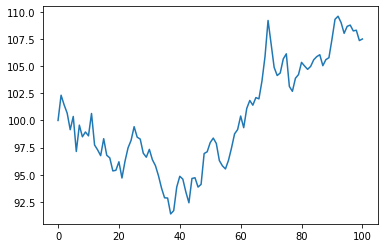
\includegraphics[width=.75\linewidth]{lecture_8_files/lecture_8_15_0.png}
    \caption{Price at $T=0$}
  \end{subfigure}
  \begin{subfigure}{.45\textwidth}
    \centering    
    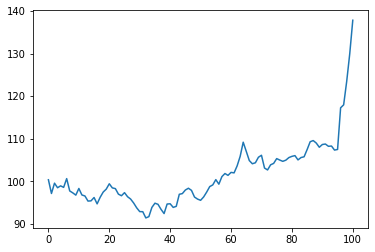
\includegraphics[width=.75\linewidth]{lecture_8_files/lecture_8_15_1.png}
    \caption{Price at $T=5$}    
  \end{subfigure}
  \newline
  \begin{subfigure}{.45\textwidth}
    \centering    
    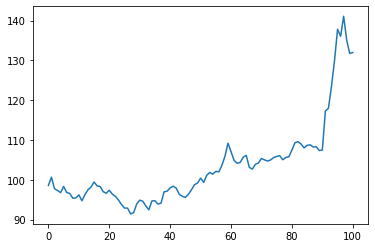
\includegraphics[width=.75\linewidth]{lecture_8_files/lecture_8_15_2.png}
    \caption{Price at $T=10$}    
  \end{subfigure}
  \begin{subfigure}{.45\textwidth}
    \centering
    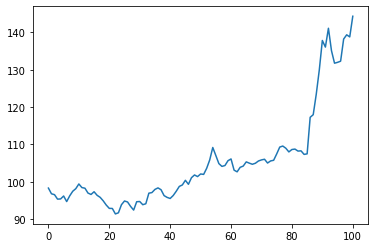
\includegraphics[width=.75\linewidth]{lecture_8_files/lecture_8_15_3.png}
    \caption{Price at $T=15$}
  \end{subfigure}
  \newline
  \begin{subfigure}{.45\textwidth}
    \centering    
    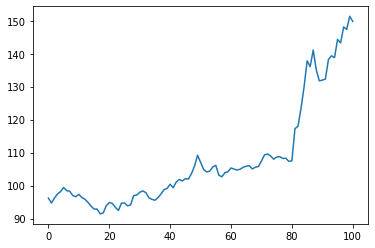
\includegraphics[width=.75\linewidth]{lecture_8_files/lecture_8_15_4.png}
    \caption{Price at $T=20$}    
  \end{subfigure}
  \begin{subfigure}{.45\textwidth}
    \centering    
    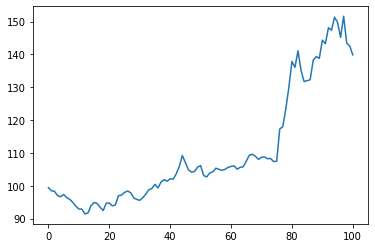
\includegraphics[width=.75\linewidth]{lecture_8_files/lecture_8_15_5.png}
    \caption{Price at $T=25$}    
  \end{subfigure}
  \newline
  \begin{subfigure}{.45\textwidth}
    \centering
    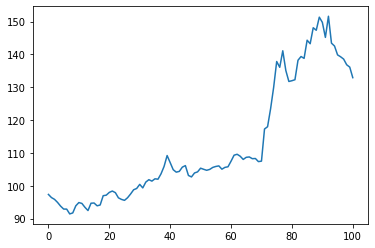
\includegraphics[width=.75\linewidth]{lecture_8_files/lecture_8_15_6.png}
    \caption{Price at $T=30$}
  \end{subfigure}
  \begin{subfigure}{.45\textwidth}
    \centering    
    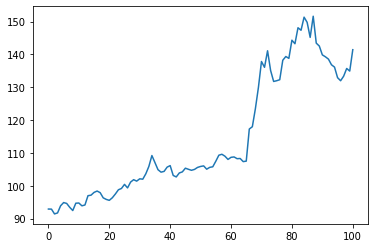
\includegraphics[width=.75\linewidth]{lecture_8_files/lecture_8_15_7.png}
    \caption{Price at $T=35$}    
  \end{subfigure}
  \newline
  \begin{subfigure}{.45\textwidth}
    \centering
    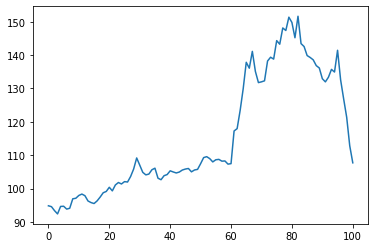
\includegraphics[width=.75\linewidth]{lecture_8_files/lecture_8_15_8.png}
    \caption{Price at $T=40$}
  \end{subfigure}
  \begin{subfigure}{.45\textwidth}
    \centering    
    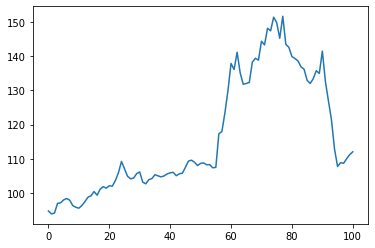
\includegraphics[width=.75\linewidth]{lecture_8_files/lecture_8_15_9.png}
    \caption{Price at $T=45$}    
  \end{subfigure}
\end{figure}
\newpage
    \begin{Verbatim}[commandchars=\\\{\}]
0  [0.96 0.00 0.03]
0  [0.66 0.00 0.33]
0  [0.96 0.00 0.03]
0  [0.93 0.00 0.06]
0  [0.93 0.00 0.06]
0  [0.56 0.00 0.43]
1  [0.00 1.00 0.00]
1  [0.00 1.00 0.00]
1  [0.00 1.00 0.00]
1  [0.00 1.00 0.00]
    \end{Verbatim}

    So at the 6th sample the CNN start recognizing the \emph{head and
shoulder} pattern in the price evolution.

    \hypertarget{exercises}{%
\subsection{Exercises}\label{exercises}}

The necessary code to run all the examples in this lesson can be found \href{https://repl.it/@MatteoSani/exercises8}{here}. Remember to install \verb|keras|, \verb|tensorflow| and \verb|mnist| modules, either using \verb|pip| or through the anaconda interface.

\begin{itemize}
\item \verb|bs_simulation.py|, simulate a large sample of calls (you can replace `call` with `put` in the file to test how the NN works with puts); 
\item \verb|bs_training.py|, perform the training of the NN on the calls, produces three samples: training, test within the phase-space and test outside the phase-space;
\item \verb|bs_testing.py|, test the NN on the testing samples;
\item \verb|digit_converter.py|, utilities to convert an handmade image into the suitable format for the CNN used in digit recognition;
\item \verb|digit_training.py|, train a CNN to recognize digits;
\item \verb|digit_testing.py|, test the digit recognition CNN on the MNIST sample and on an handmade digit (remember to set the correct file name in this second case);
\item \verb|techana_simulation.py|, simulate many time series with no feature, with \emph{head-and-shoulders} and with \emph{triangle};
\item \verb|techana_training.py|, train a CNN to search for patterns in time series;
\item \verb|techana_testing.py|, test the performance of the CNN for techical analysis.
\item \verb|testing_techana_frames.json|, time series to check the CNN for techical analysis.  
\end{itemize}

If you have issues in running one of all the files, please contact me at \href{mailto:matteosan1@gmail.com}{matteosan1@gmail.com}.

\hypertarget{exercise-8.1}{%
\subsubsection{Exercise 8.1}\label{exercise-8.1}}

Try to repeat all the example shown during the lesson.

\hypertarget{exercise-8.2}{%
\subsubsection{Exercise 8.2}\label{exercise-8.2}}

Using the same code illustrated above, test the ANN to recognize digits
with your own handwriting (e.g.~try to exagerate some feature to fool
the NN, or even pass it letters instead of digits and interpret the
results).

\hypertarget{exercise-8.3}{%
\subsubsection{Exercise 8.3}\label{exercise-8.3}}

Taking as example the pricing NN trained on call, try to price put
options.


    % Add a bibliography block to the postdoc
    
    
    
\end{document}
